\chapter{Background \& Related Work}\label{chapter:background}

\section{Ethereum}\label{sec:ethereum}
Ethereum is considered to be a distributed transaction-based state machine  \citep{wood_2014}. There are two key components that enable Ethereum’s operation. The Ethereum Virtual Machine (EVM), which is a Turing-complete virtual machine with a simple stack-based architecture and the Ethereum blockchain, an append-only timestamped data structure where transactions and relevant information are stored. Each node that participates in the Ethereum network runs an instance of the EVM and holds a copy of the blockchain. State transitions are caused by the execution of transactions, which may result either in a transmission of value between accounts or an execution of EVM code associated with an account. Such code, known as SC, is essentially an immutable computer program that runs on top of the Ethereum protocol. Typically, SCs are written in high level programming languages, primarily in Solidity  \citep{solidity}, but must be compiled to a series of bytecode instructions in order to be executed by the EVM.

Since Ethereum aims to provide the necessary infrastructure for all kinds of applications, having a persistent memory area for the needs of the applications, is crucial. Indeed, every SC owns an autonomous memory area called storage, where data can be saved.

\subsection{Gas}\label{sec:gas}
Every transaction that takes place on the Blockchain is stored and verified by all nodes of the network, burdening it. Therefore, to avoid unnecessary abuse of network resources, transactions are associated with a fee. In the case of Bitcoin, this is determined by the Miners, depending on the network load. In Ethereum, since beyond the mere transfer of cryptocurrencies, execution of code and data storage are supported, a different strategy has been adopted.

A transaction in Ethereum, whether it's a simple transfer of Ether or a complex smart contract function call, involves the execution of operations. These operations are subject to a fee which is predetermined  \citep{wood_2014} and paid in gas, the fundamental cost unit in Ethereum. Basically, the more resources a particular operation consumes, the more gas it costs. Without a measure like gas, someone could deliberately spam the network with complex operations, causing it to slow down.

\begin{table}[htbp]
\caption{Gas costs for some basic operations up to Muir Glacier fork \citep{wood_2014}.}
\label{table:operations_cost}
\resizebox{\textwidth}{!}{%
\begin{tabular}{@{}lrl@{}}
\toprule
 \textbf{Name} & \textbf{Value} & \textbf{Description} \\ \midrule
 $G_{\mathrm{sset}}$ & 20000 & Paid for an {\small SSTORE} operation when the storage value is set to non-zero \\
 && from zero. \\
 $G_{\mathrm{sreset}}$ & 5000 & Paid for an {\small SSTORE} operation when the storage value's zeroness remains \\
 && unchanged or is set to zero. \\
 $G_{\mathrm{create}}$ & 32000 & Paid for creating a new account with associated code. \\
 $G_{\mathrm{codedeposit}}$ & 200 & Paid per byte for a {\small CREATE} operation to succeed in placing code into state. \\
%  $G_{\mathrm{newaccount}}$ & 25000 & Paid for a {\small CALL} or {\small SELFDESTRUCT} operation which creates an account. \\
%  $G_{\mathrm{memory}}$ & 3 & Paid for every additional word when expanding memory. \\
 $G_\text{txcreate}$ & 32000 & Paid by all contract-creating transactions after the {\textit{Homestead} transition}.\\
 $G_{\mathrm{txdatazero}}$ & 4 & Paid for every zero byte of data or code for a transaction. \\
 $G_{\mathrm{txdatanonzero}}$ & 16 & Paid for every non-zero byte of data or code for a transaction. \\
 $G_{\mathrm{transaction}}$ & 21000 & Paid for every transaction. \\
 $G_{\mathrm{log}}$ & 375 & Partial payment for a {\small LOG} operation. \\
 $G_{\mathrm{logdata}}$ & 8 & Paid for each byte in a {\small LOG} operation's data. \\
 $G_{\mathrm{logtopic}}$ & 375 & Paid for each topic of a {\small LOG} operation. \\ \bottomrule
\end{tabular}
}
\end{table}

Gas cannot be used by users to pay for a transaction directly. In practice, prior to a transaction’s execution, a certain amount of gas, known as gasLimit, is purchased with Ether at a certain gasPrice. Both gasLimit and gasPrice are specified by the sender. After the transaction is completed, any unused gas are converted back to Ether, at the rate they were purchased and returned to the sender. The Ether corresponding to the gas consumed constitutes the fee of the transaction and is granted to the \hl{miner/validator} as a reward. 
% TODO: add a footnote with this informing about EIP-1559. Also for intrinsic gas and intrinsic cost
% (\hl{is taken into account while calculating the transaction's fee which is granted to..})

In the context of a transaction, gasLimit indicates the amount of gas the sender is willing to spend. A transaction will fail if a) the gasLimit is lower than the intrinsic gas \textit{g0} (see fig. \ref{fig:intrinsic_cost}), b) the sender's balance cannot cover the intrinsic cost \(v0 = gasPrice * gasLimit + transferredEther\), or the gasLimit is not sufficient for the execution of the operations associated with it. In the first two cases, the transaction is considered invalid from the beginning and is not executed. In the last case, the transaction is executed until the available gas are exhausted. This burdens the network's resources, so the fee resulting from the consumed gas is compensated to the \hl{Miner/validator}. Note that any changes that have been made during the execution of a failed transaction are reversed. As is obvious, the correct determination of gasPrice and gasLimit values is necessary for the successful completion of transactions.

\begin{figure}[h!]
\begin{small}
\setlength{\mathindent}{0pt}
\begin{align}
g_0 \equiv {} & \sum_{i \in T_{\mathbf{i}}, T_{\mathbf{d}}} \begin{cases} {G_{\mathrm{txdatazero}}} & \text{if} \quad i = 0 \\ {G_{\mathrm{txdatanonzero}}} & \text{otherwise} \end{cases}
\nonumber {} & + \begin{cases} {G_{\mathrm{txcreate}}} & \text{if contract creation} \\ 0 & \text{otherwise} \end{cases}
\nonumber {} & + {G_{\mathrm{transaction}}} \\
\nonumber
% \nonumber {} & + \sum_{j = 0}^{\lVert T_{\mathbf{A}} \rVert - 1} \big( G_{\mathrm{accesslistaddress}} + \lVert T_{\mathbf{A}}[j]_{\mathbf{s}} \rVert G_{\mathrm{accessliststorage}} \big)
\end{align}
\end{small}
\caption{Intrinsic gas calculation up to Muir Glacier fork. $T_{\mathbf{i}},T_{\mathbf{d}}$ refer to the transaction's data and contract initialization code.}
\label{fig:intrinsic_cost}
\end{figure}

The existence of this limit arises from a problem known in computer science as the Halting Problem \citep{burkholder_1987}. A brief description of it is: given an arbitrary program and an input, it is impossible to know in advance if the program will complete or will "run" indefinitely. Imposing a limit on the number of operations that can be executed during a transaction, prevents the EVM from getting stuck in intentional (by malicious users) or unintentional infinite loops.

In addition to transactions, each block has an equivalent limit that bounds the total gas that can be consumed by the transactions included in it. This in turn limits the number of transactions that can be included in a block, thus regulating the size of the blocks.

Utilizing a contract’s storage also results in a gas fee. In particular, the cost of writing data on storage is proportional to the data’s size and as depicted in table \ref{table:operations_cost}, especially high, as a means to keep the distributed database as small as possible. Consequently, storage space within the Ethereum network is a valuable resource and it should be used sparingly to store what is required for the SC's proper operation. Obviously, this limits drastically the amount of data an application can store on Ethereum.

\subsection{Refunds}\label{sec:gas}


\subsection{Forks \& EIPs}\label{sec:gas}
In blockchain technology, a \textit{fork} refers to a split in the chain of blocks. For instance, this can happen when two different miners produce a valid block at nearly the same time. This ambiguity is resolved when subsequently added blocks render one as the longest chain. However, forks can occur due to intentional changes in the rules of the blockchain protocol. 

The introduction of changes and new rules lead to a split in the network. If the changes are backwards compatible, meaning that new blocks can be produced based on either the new rules or the old ones, the fork is called \textit{soft} and nodes that did not upgrade their software can still participate in the network and process transactions \citep{etherscaninformationcenter_2022}. On the other hand, a \textit{hard} fork happens when major changes that break backward compatibility are implemented. In that case, all nodes must adopt the upgrades and abide by the new rules, else a permanent network split could occur. A notable example of this in Ethereum's history was the DAO fork \citep{ethereumfoundation_2023} which was enforced in response to the DAO attack \citep{vujicic_2018} and lead the creation of Ethereum Classic, as a part of the network decided to continue following the old rules.

In the context of Ethereum, the changes introduced by the forks are typically derived from Ethereum Improvement Proposals (EIPs), which suggest improvements to the underlying protocol. In short, they are technical documents that propose enhancements or introduce new features and processes. 

\begin{figure}[htbp]
\centerline{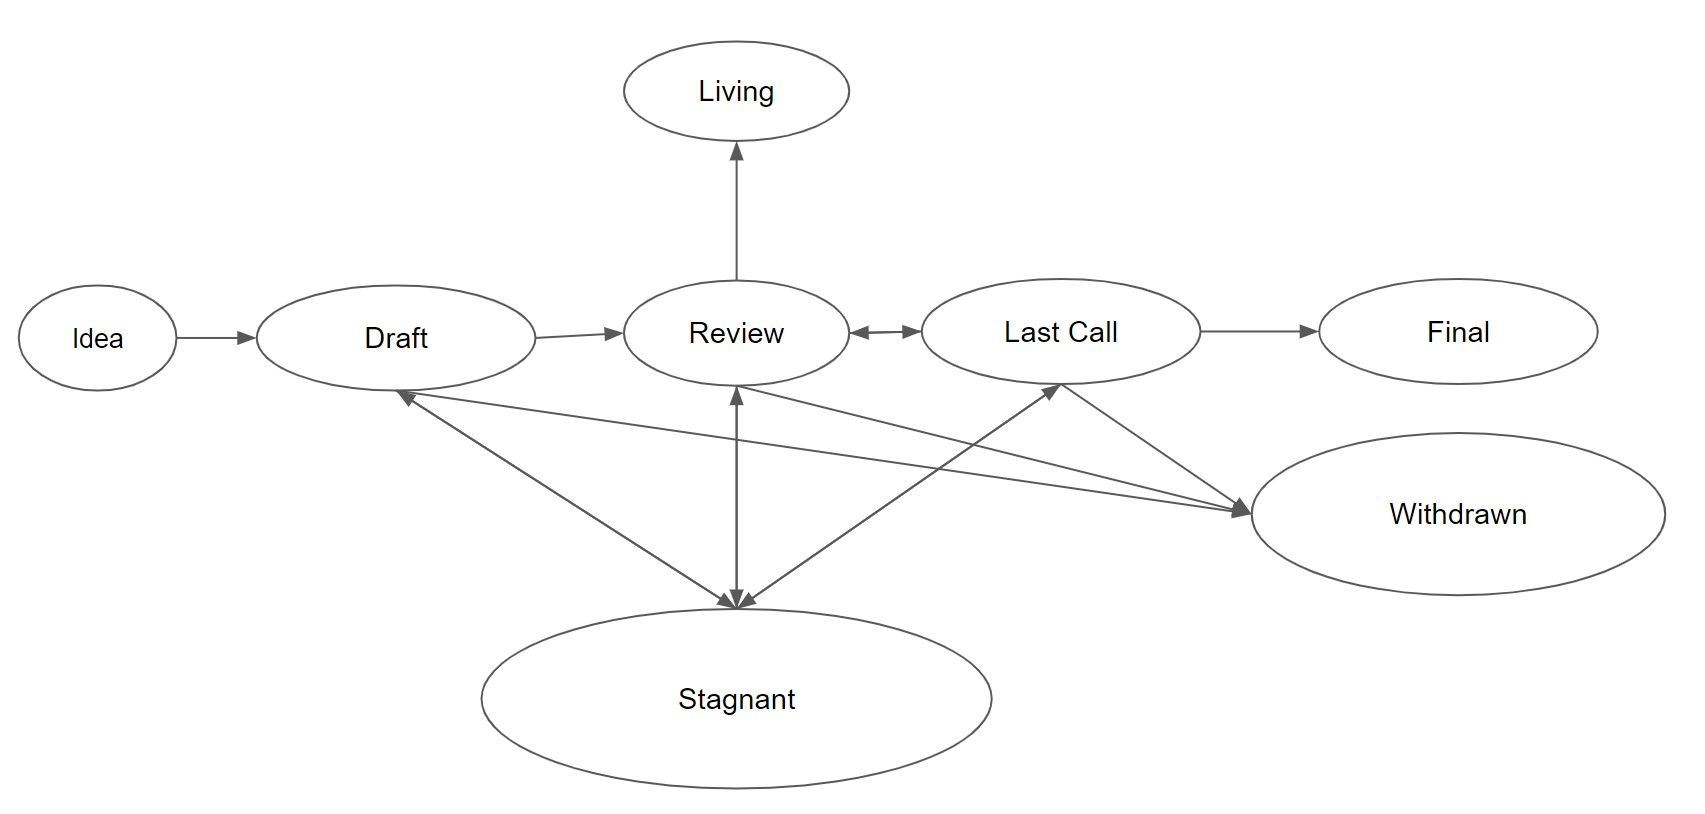
\includegraphics[width=\textwidth]{figs/eip_stages.jpg}}
\caption{EIP standardization process \citep{ethereumfoundation_2023b}.}
\label{fig: eip_stages}
\end{figure}

EIPs are part of an open-source collaboration process. They offer a formal way for individuals in the Ethereum community to suggest changes and upgrades to the network. Each EIP must go through a process of discussion and approval by the Ethereum community. The process is illustrated in fig. \ref{fig:eip_stages} and involves initial drafting, reviewing, modifications, and eventually, if there is sufficient consensus among the community, the EIP is finalized and the changes can be implemented in the Ethereum protocol. 

% There are several types of EIPs, including:
% Standard Track EIPs - these relate to changes to the network protocol itself, such as changes to block or transaction validity rules, proposed application standards/conventions, and changes/upgrades to networking protocols.
% Meta EIPs - these propose design issues, general guidelines or information to the Ethereum community, or describe a new feature for Ethereum or its processes or environment.
% Informational EIPs - these describe an Ethereum design issue, or provide general guidelines or information to the Ethereum community, but do not propose a new feature.
% ERC (Ethereum Request for Comments) EIPs - these are application-level standards and conventions, including contract standards like the well-known ERC-20 and ERC-721, which provide rules for Ethereum token contracts.

In Ethereum, every fork that takes place includes a set of EIPs that each Ethereum client must implement to remain in consensus with the rest of the network \citep{ethereumfoundation_2023a}. This requirement ensures that all client developers adhere to the same rules, thereby maintaining network integrity.

Below we discuss some of the EIPs that were implemented in view of the Berlin and London forks.

\paragraph{EIP-2929}\label{par:eip_2929_cold_warm}

EIP-2929, included in Berlin fork, proposes an increase in gas costs for certain opcodes and also reforms  to prevent potential denial-of-service (DoS) attacks \citep{buterin_eip_2929}. Additionally, it outlines the adjustments that need to be made to the SSTORE and SELFDESTRUCT metering mechanisms in order to avoid unfair rates due to the SLOAD operations entailed in such operations.

Since our research revolves mainly around data management, we do not elaborate on how this EIP affect the *CALL opcode family, EXT* opcode family and the SELFDESTRUCT metering mechanism. Thus, below we present only the reformed SSTORE metering mechanism. As reference, the corresponding Geth’s implementation was used  \citep{ethereum_2022}.

\vspace{0.2cm}
\noindent
\textsc{sload} cost modification:
   \begin{itemize}[topsep=0pt, itemsep=0pt]
     \item  \textsc{warm\_sload}: charge 100 gas if slot has already been accessed in current execution context.
     \item  \textsc{cold\_sload}: charge 2100 gas if slot has not been accessed in current execution context.
   \end{itemize}
   
\vspace{0.2cm}
\noindent
 \textsc{sstore} cost modification:
   \begin{itemize}[topsep=0pt, itemsep=0pt]
     \item  Initialize a slot:
     \begin{itemize}[topsep=0pt, itemsep=0pt]
        \item If slot is not already accessed: charge \textsc{cold\_sload} + \textsc{sstore} = 2100 + 20000 = 22100
        \item If slot is already accessed: charge \textsc{sstore} = 20000
     \end{itemize}
   \end{itemize}
   
   \begin{itemize}[topsep=0pt, itemsep=0pt]
     \item  Update a slot: 
     \begin{itemize}[topsep=0pt, itemsep=0pt]
        \item If slot is not already accessed: charge \textsc{cold\_sload} + \textsc{(sstore\_reset - cold\_sload)} = 5000
        \item If slot is already accessed: charge \textsc{(sstore\_reset - cold\_sload)} = 5000 – 2100 = 2900
     \end{itemize}
   \end{itemize}
   
   \begin{itemize}[topsep=0pt, itemsep=0pt]
     \item  Overwriting a slot with the same value (no-op):
     \begin{itemize}[topsep=0pt, itemsep=0pt]
        \item If slot is not already accessed: charge \textsc{(cold\_sload + warm\_sload)} = 2100 + 100 = 2200
        \item If slot is already accessed: charge \textsc{warm\_sload} = 100 
     \end{itemize}
   \end{itemize}


\paragraph{EIP-2930}\label{par:eip_2930_access_list}
EIP-2930  \citep{buterin_eip_2930} adds a new transaction type and introduces the notion of an optional AL, a list of entries with each entry being a tuple of an account address and a list of storage keys that the transaction plans to access. This essentially enables a user to\emph{``warm-up''} the accounts and storage slots they plan to access, at a discounted cost. 

The cost for warming up each account address is $G_{\mathrm{accesslistaddress}} = 2400$ and 
$G_{\mathrm{accessliststorage}} = 1900$ for each storage key, and is paid upfront. As a result, the calculation of the intrinsic gas \textit{g0} changes to:

\begin{small}
\setlength{\mathindent}{0pt}
\begin{align}
g_0 \equiv {} & \sum_{i \in T_{\mathbf{i}}, T_{\mathbf{d}}} \begin{cases} {G_{\mathrm{txdatazero}}} & \text{if} \quad i = 0 \\ {G_{\mathrm{txdatanonzero}}} & \text{otherwise} \end{cases}
\nonumber {} & + \begin{cases} {G_{\mathrm{txcreate}}} & \text{if contract creation} \\ 0 & \text{otherwise} \end{cases}
\nonumber {} & + {G_{\mathrm{transaction}}} 
\nonumber
\end{align}
\begin{align}
& + \sum_{j = 0}^{\lVert T_{\mathbf{A}} \rVert - 1} \big( G_{\mathrm{accesslistaddress}} + \lVert T_{\mathbf{A}}[j]_{\mathbf{s}} \rVert G_{\mathrm{accessliststorage}} \big)
\intertext{Where $T_{\mathbf{i}},T_{\mathbf{d}}$ refer to the transaction's associated data and initialization EVM-code and $T_{\mathbf{d}}$ to the access list.} \nonumber
\end{align}
\end{small}

% TODO: is this necessary?
Considering table \ref{table:operations_cost}, a more convenient representation of the intrinsic gas that must be paid for a contract call is:
\begin{flushleft}
\centering
$g_0 \equiv 21000 + 16 * \textsc{non\_zero\_bytes} + 4 * \textsc{zero\_bytes} + 1900 * \textsc{storage\_key\_count } + 2400 * \textsc{address\_count}$
\end{flushleft}

All the accounts and storage slots specified in the AL are considered “warmed up” and consequently SLOAD, *CALL, BALANCE, EXT* operations on them are charged as if they were already accessed, in accordance with EIP-2929. Table~\ref{table:access_list} is a simplified representation of the access-cost when an AL is or is not utilized.

\begin{table}[htbp]
\caption{Impact of the Optional Access List}
\label{table:access_list}
\resizebox{\textwidth}{!}{%
\begin{tabular}{@{}lll@{}}
\toprule
 & \textbf{No access list} & \textbf{Access list}  \\ \midrule
\textbf{Account} & \begin{tabular}[c]{@{}l@{}}2600 for first access + \\ 100 for each subsequent access\end{tabular} & \begin{tabular}[c]{@{}l@{}}2400 to be included in the AL + \\ 100 for each access\end{tabular} \\
\textbf{SLOAD} & \begin{tabular}[c]{@{}l@{}}2100 for first access + \\ 100 for each subsequent access\end{tabular} & \begin{tabular}[c]{@{}l@{}}1900 to be included in the AL + \\ 100 for each access\end{tabular}
\\
\textbf{SSTORE} & \begin{tabular}[c]{@{}l@{}}22100 for each initialization\end{tabular} & \begin{tabular}[c]{@{}l@{}}1900 to be included in the AL + \\ 20000 for each initialization\end{tabular}
\\
\textbf{SSTORE} & \begin{tabular}[c]{@{}l@{}}5000 for each update\end{tabular} & \begin{tabular}[c]{@{}l@{}}1900 to be included in the AL + \\ 2900 for each update\end{tabular}
\\
\textbf{SSTORE} & \begin{tabular}[c]{@{}l@{}}2200 for each each update (same value)\end{tabular} & \begin{tabular}[c]{@{}l@{}}1900 to be included in the AL + \\ 100 for each update (same value)\end{tabular}
\\* \bottomrule

\end{tabular}%
}
\end{table}
    
The main objective of this EIP is to mitigate risks introduced by the refined gas metering mechanism described in paragraph \ref{par:eip_2929_cold_warm}. For instance, an external function call that is allowed to consume a specific amount of gas (see fig. ) might be rendered un-callable due to increased gas costs we discussed previously. By warming up these addresses, such scenarios can be dealt with. 

\begin{figure}[htbp]
\centerline{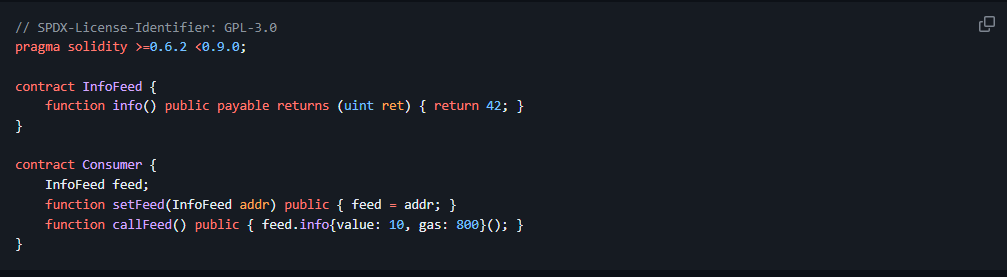
\includegraphics[width=\textwidth]{figs/solidity_external_function.png}}
\caption{Example of an external function call with specified gas.}
\label{fig: external_function_call}
\end{figure}

% \paragraph{EIP-1559}\label{par:eip_1559_gas_limit}

\paragraph{EIP-3529}\label{par:eip_3529_refund}
This EIP \citep{buterin_eip_3529} was a part of the London fork and introduced the following changes to the Ethereum gas refund mechanism:

\begin{itemize}
  \item Removal of gas refunds for the \textsc{selfdestruct} operation
  \item Reduction of gas refunds for clearing a storage slot from 15000 gas to \\ \textsc{sstore\_reset + access\_list\_storage\_key = 4800} gas.
  \item Reduction of the maximum refund that the sender is eligible to get, from half to a fifth of the total gas used.
\end{itemize}

Gas refunds were initially introduced to incentivize developers to clear storage slots and delete contracts that are no longer required in order to lower the blokcain's size. Despite this motivation, the practice has not been widely adopted and the harmful consequences seem to outweigh the benefits \citep{buterin_eip_3529}.

Firstly, refunds gave rise to exploitations such as the GasToken \citep{gastokenproject_2018}. The idea is that users can save on transaction fees by reserving storage slots with data or creating contracts when gas prices are low and freeing slots or deleting the contracts when gas prices are high in order to benefit from the refund. Obviously, this results in needless increase of the blockchain's state size. Secondly, since gas refunds allow for more gas to be used within the same block, they have affected block size variance.

The changes proposed in the described EIP do not fully negate the concept of refunds, but they ensure that the total refundable amount is restricted to a level such that current exploits are not viable.

The revised refund mechanism limits the overall refund amount
\section{Distributed File Systems}\label{sec:dfs}
In peer-to-peer distributed file systems, participating nodes share their resources to store and access all kinds of content. Nowadays, IPFS and Swarm are two of the most promising distributed file systems. Both have implemented, evolved, and connected widely researched techniques found in the domain of distributed systems. They aim to be platforms where users can trust the content they receive, without trusting the peers that provide it.

Unlike centralized systems where data is located and accessed based on its physical location (i.e. server address), distributed file systems utilize content addressing. Content addressing \citep{trautwein_2022} refers to a mechanism where data is identified and retrieved based on its content, rather than its location. Some features inherent to content addressing are:

\begin{itemize}
    \item \textbf{Decentralization and performance}: Nodes on the network can locate and retrieve data from any other node in the network that has the data, supporting decentralization and reducing overall latency.
    \item \textbf{Immutability and Integrity}: Immutability is a fundamental characteristic of content addressing. Once data is stored and its content-based address is generated, typically using a cryptographic hash function, any interference with the data would change its address. This ensures that the data cannot be altered without detection, reinforcing data integrity.
    \item \textbf{Deduplication}: Within a node's storage space, data is identified by its content. Therefore, even if the same data is added multiple times only one copy will be retained, saving storage space and improving system efficiency.
\end{itemize}

Beyond the benefits derived from content addressing, the decentralized nature of distributed file systems like IPFS and Swarm offers several advantages over centralized solutions \citep{daniel_2022, ipfs_docs_1}. Firstly, they achieve data redundancy, ensuring that content is replicated across multiple nodes, often by means of data caching. This redundancy enhances fault tolerance, as usually, the loss of a single node does not result in data loss. Furthermore, having multiple copies of data distributed across the network, the likelihood of data being accessible increases.

Except for fault tolerance and availability, data caching plays a vital role in improving the overall retrieval performance of distributed file systems. This is apparent in systems like IPFS and Swarm, where recently accessed data is cached. This means that when a node requests a specific piece of data, if it is cached by a nearby node, it can be retrieved more quickly, as it doesn't need to traverse the entire network. As one might expect, popular content tends to be replicated extensively across the network, reducing its retrieval latency.

Another key feature of IPFS and Swarm is that they are resilient against censorship. As already mentioned, data in these platforms is addressed by its content and isn't stored in a single location or controlled by a single entity. Instead, it's distributed across multiple nodes which makes it extremely difficult for an individual party to censor information. Once data is uploaded and as long as at least one node on the network has a copy of the content, it can be accessed from any other node, promoting freedom in terms of access to information \citep{IPFS_team_2017}.

In summary, distributed file systems present significant advantages over traditional centralized storage systems. By employing content-based addressing, they enable deduplication and location independence while enforcing data integrity. Also, since they offer decentralized access to data and leverage data caching, they provide data redundancy, censorship-resistance, availability and efficient retrieval, even in the face of node failures or network disruptions.

\subsection{IPFS}\label{sec:ipfs}
% TODO: data or content
The InterPlanetary File System (IPFS) is an open-source, peer-to-peer network that aims to \hl{revolutionize/redefine} data storage and delivery through its innovative content-addressable system \citep{benet_2014}. As an open, permissionless system, IPFS is accessible to anyone, allowing participants to host and download data from other peers. 

Data, when uploaded, is split into chunks and is stored by a small set of nodes - the initial uploader and any nodes that download and cache the data - known as \textit{providers} who make the data available to other peers. Due to its decentralized architecture, IPFS ensures there's no single point of failure and operates effectively without the need for mutual trust between nodes.

A fundamental component of IPFS is the Kademlia based Distributed Hash Table (DHT) \citep{maymounkov_2002} that serves as a decentralized catalog and navigation system, routing content requests to data providers in the network. Essentially, it maintains mappings of data identifiers to peers and peers to their network addresses. Kademlia is known \citep{benet_2014} for its efficient lookup through massive networks and thereby facilitates quick content discovery and peer communication. The actual peer-to-peer connectivity as well as most of IPFS' networking functionality is handled by libp2p, a reusable networking library which was initially developed as part of the IPFS project. Libp2p \citep{libp2p_2023} supports a variety of transport protocols and ensures encrypted communication between peers, thereby promoting security and flexibility.

In the following paragraphs, we describe key components of IPFS’ design concentrating specifically on the those that align with our research objectives. It is worth noting that since IPFS and its subsystems are under continuous development, details of the design may change over time.

\paragraph{Nodes in IPFS}\label{par:nodes_ipfs}
To join the IPFS network, a node initially contacts bootstrap nodes. These bootstrap nodes provide the new node with information about other peers in the network, so that it is able to form its \textit{swarm} or set of known peers. After joining the network, the node generates a unique \hl{peerID} that serves as the node's identifier and is derived from the hash of its public key.

\begin{figure}[htbp]
    \centerline{\includegraphics{figs/Multiaddress.png}}
    \caption{Structure of a Multiaddress. \citep{trautwein_2022}}
    \label{fig:multiaddress}
\end{figure}

Each node maintains part of the global DHT that contains, among others, peer records that map a \hl{peerID} to a set of Multiaddresses at which the peer may be reached \citep{schmahmann_2020}. Multiaddresses \citep{multiaddress_2023} are self-describing, human-readable, and as shown in fig. \ref{fig:multiaddress}, except for the node's \hl{peerID} they encode information about how the peer can be reached in the underlying network, e.g the network address (such as an IPv4, IPv6 address), the transport protocol (such as TCP, UDP, QUIC) and the port number. Basically, Multiaddresses enable nodes to communicate with each other over different network protocols and address types.

\paragraph{Storing content}\label{par:storing_ipfs}
When content is added to IPFS, it is split into chunks, each having a default size of 256 kB (configurable). A unique Content Identifier (CID) is then assigned to each chunk. This CID is created by hashing the chunk's content and appending relevant metadata. As of now, there are two CID versions implemented. The CID v1 format \citep{multiformat}, which will be the default in the near future, consists of four parts

% \[\textsc <cidv1> ::= <multibase><multicodec-version><multicodec-content-type><multihash>\]

\begin{flushleft}
\centering
$\textsc <cidv1> ::= <multibase><multicodec-version><multicodec-content-type><multihash>$
\end{flushleft}

while CID v0 contains only the \(\scriptstyle <multihash>\), which is always a SHA-256 multihash \citep{multiformat}, i.e., a 34-byte hex array with the leading bytes [0x12, 0x20], used to denote the hash function and the hash digest’s size, followed by the hash digest. The rest are implicitly assumed to be (base58btc - cidv0 - dag-pb).

The leading three parts of the CID V1, namely, \(\scriptstyle <multibase>\), \(\scriptstyle <multicodec-version>\), and \(\scriptstyle <multicodec-content-type>\), denote the base in which the CID was encoded, its version, and the type of data it refers to, respectively. Applying base encoding to a CID aims to minimize its overall length. The \(\scriptstyle <multihash>\) represents the hash function that is applied on the binary data along with size of the resulting hash digest. It enables support for multiple hash functions, thus providing flexibility, future-proofing, interoperability and security. % TODO: maybe add citation

\begin{figure}[htbp]
    \centerline{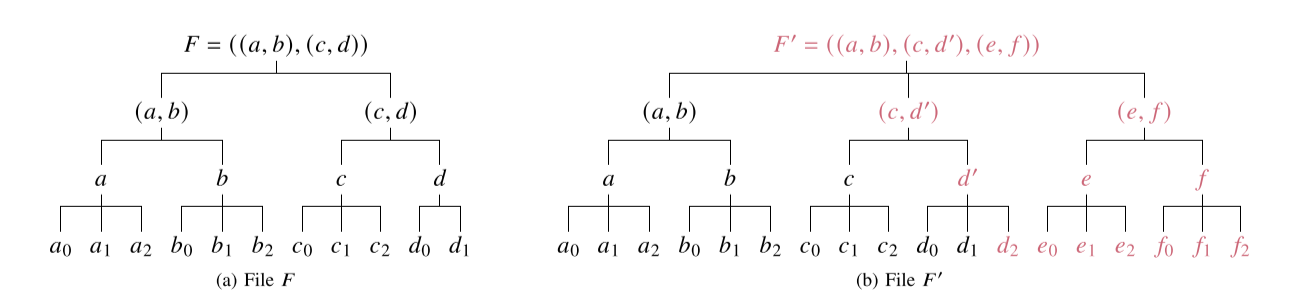
\includegraphics[width=\textwidth]{figs/deduplication.png}}
    \caption{Concept of deduplication. \citep{daniel_2022}}
    \label{fig:deduplication}
\end{figure}

The CIDs of individual chunks are organized in a Merkle Directed Acyclic Graph (DAG) which represents the original content's structure. A Merkle DAG \citep{benet_2014}, is similar to a Merkle tree but without the balance requirement. It allows for a node to have multiple parents, enabling deduplication of chunks (see fig. \ref{fig:deduplication}). This leads to efficient storage and bandwidth usage as the same content doesn't need to be stored or transmitted more than once \citep{trautwein_2022}. The root node of the Merkle DAG is the CID that is used to identify the content.

CIDs are immutable due to their hash-based structure, ensuring that the content cannot be altered without modifying its CID. This enables self-verification, as the CID can be compared with the hash of the content itself for authenticity.

\paragraph{Providing content}\label{par:providing_ipfs}
Revisiting our previous discussion in paragraph \ref{par:nodes_ipfs}, IPFS uses a DHT as a core component of its content routing system. Each node participating in the IPFS network maintains a subset of the DHT that stores three types of key-value pairs, provider records, IPNS records, peer records \citep{schmahmann_2020}. IPNS records are outside the scope of this work and therefore we do not elaborate on them. Peer records are described in paragraph \ref{par:nodes_ipfs}. Provider records map data identifiers to peers that can serve the specific content.

When uploading content, the node stores it locally and then generates a provider record that associates the content's CID with its own \hl{PeerID}. This record is then disseminated into the DHT, signaling to the network that the node can provide the content. The provider record is strategically stored in the DHT segments of the \textit{k} \hl{(\textit{k}= 20)} nodes that are closest to the hash of the content's CID. Closeness, is represented by the XOR distance \citep{maymounkov_2002} of the \hl{node's id} and the CID's hash. By replicating the provider record across \textit{k} nodes, fault-tolerance and availability are enhanced. 

For the upload process to be completed, the node also needs to broadcast its peer record, so that when other nodes wish to retrieve the content, they can learn of its Multiaddresses and establish a connection.

\paragraph{Retrieving content}\label{par:retrieving_ipfs}
% TODO: add citation for bitswap
In IPFS, when a node wants to retrieve content associated with a certain CID, it initially uses the Bitswap protocol to query its direct peers.  If one of these peers has the content, they return it immediately. If unsuccessful, \hl{(after a timeout of one second)} the node leverages the DHT for content discovery.

%TODO: improve the paragraph 
As already mentioned in the previous paragraph , the nodes closest to the requested CID are most likely to hold information about content providers. In this respect, the node forwards a request for the content to \textit{x} \hl{(\textit{x}= 3)} of his peers that are closest to the CID. Based on the circumstances, these nodes either: 1) respond with the requested content (if they have it), 2) return a provider record that points to the peer that hosts the content, 3) suggest other peers closer to the desired CID. The latter is a process that is repeated until either the content or a provider record is obtained, e.g. the node queries the suggested peers, and if they in turn suggest other peers, the node asks those peers, and so forth.

Next, the node, now aware of the \hl{PeerID(s)} hosting the content, queries the DHT again to obtain the corresponding peer records that contain the Multiaddresses of the peers. Note that each node maintains a separate list of peers that it has recently interacted with, which it queries prior to resorting to the DHT, in order to reduce the lookup time.

With the Multiaddresses at hand, the node can now connect to the peers that have the content. Content retrieval then takes place via Bitswap and upon delivery the user can verify the integrity of the received content by reconstructing the CID, ensuring it matches the original request.

\paragraph{Caching}\label{par:caching_ipfs}
Nodes on the IPFS network, have a built-in caching mechanism that allows them to automatically cache content they have recently accessed. When nodes fetch data, they always store a copy in their local cache.

While content is present in a node's local storage, it can be served to other nodes who might request it, reducing retrieval latency, e.g. fetching a cached block from a neighboring node eliminates the overhead of a network traversal. This becomes particularly effective when dealing with popular content that is cached by multiple nodes, as the likelihood that the content is retrieved from nearby sources increases.

Cached content remains available until it is garbage collected. Garbage collection in the field of computer science refers to a process that identifies and removes content that is no longer in use, based on various strategies \citep{gc_2023}. In the case of IPFS, the garbage collection strategy involves identifying and discarding all \emph{``unpinned''} blocks \citep{ipfs_docs_2}. \hl{Explicitly pinned content and files added to the Mutable File System (MFS) - implicitly pinned content - are protected against garbage collection.}

\subsection{Swarm}\label{subsection:swarm}
Swarm is a groundbreaking, peer-to-peer distributed file system developed by the Ethereum Foundation. This technology aims to provide a decentralized and resilient storage layer for the decentralized web. As Tron suggests \citep{tron_2021}, with the Ethereum blockchain as the CPU of the world computer, Swarm is best thought of as its \emph{``hard disk''}. The combination of distributed computing provided by Ethereum and distributed storage offered by Swarm allows for the development of fully decentralized applications. Such DApps benefit from the high availability, zero-downtime, censorship resistance, and integrity offered by Swarm's secure, reliable, and scalable infrastructure.

Swarm utilizes peer-to-peer networking, which is facilitated by libp2p, and distributed hash tables to create a content-addressable network that allows users to upload and retrieve content in a decentralized and fault-tolerant manner. It resembles traditional cloud hosting \citep{swarmwiki_2019}, except that the content is not stored in a central server, but is split into fixed-size chunks, which are then distributed to nodes throughout the network. To achieve this the Swarm team developed an innovative storage model called Distributed Immutable Store for Chunks (DISC) \citep{swarm_team_2021} that aims to provide more efficient data management and retrieval than the traditional DHT.

In order to ensure that nodes are motivated to store and share the data for which they are responsible, Swarm incorporates a built-in incentive system. Even though this aspect guarantees data availability and is crucial for the sustainability of the network in general, it falls outside the scope of our research. Our focus in this work primarily revolves around Swarm's structural design, data distribution, and content retrieval methods.

\paragraph{Content Addressing}\label{par:chunks_swarm}

Chunks are the basic storage units in Swarm and default to a size of 4kB. Currently two types of chunks are supported: content-addressed chunks and single-owner chunks \citep{swarm_team_2021}. We focus on the former.

\begin{figure}[htbp]
    \centering
    \resizebox{1\textwidth}{!}{
    \tikzset{
level/.style={
  sibling distance={(width("$H^126$")+4pt)},
  level distance=15mm,
  line width=.5pt,
},
mtnode/.style={
  minimum width={width("$H^126$")+2pt},
  minimum height={.7cm},
  inner sep=2pt,
  outer sep=2pt,
  rectangle,
  rounded corners=1pt,
  draw,
  line width=.7pt
},
% edge from parent/.style={draw=none},
mtedge/.style={grow=down,draw=none,<-, edge from parent/.style={draw}},
link/.style={draw=none, edge from parent/.style={draw=none}},
mtedgeadj/.style={mtedge, shorten >=10pt  },
mpedge/.style={mtedge, line width=.7pt,densely dashed},
ellip/.style={draw,loosely dotted, shorten >=5mm, thick,<-, edge from parent/.style={draw}},
bubble/.style={minimum height={1cm}, draw=none, align=center},
data/.style={mtnode,fill=gray!50,line width=.7pt},
mppath/.style={mtnode,line width=.7pt},
mpext/.style={mtnode,line width=.7pt},
mpdata/.style={data,line width=.7pt},
mpdataext/.style={data,line width=.7pt}
}

\begin{tikzpicture}
                  % level 7
\node[mtnode](bmtroot){$H_R$}
  child[<-,grow=left,level distance=3cm] { node[bubble] (ash) {BMT Chunk Hash}  }
  child[grow=down]{ node[mtnode] at (-2,0)(root) {$1337$}
    child[<-,grow=left,level distance=3cm] { node[bubble] (ash) {8 byte span}  }
  }
  child[grow=down]{ node[mtnode] at (2,0) (root) {$H^7_0$}
                  % level 6
  child[<-,grow=right,level distance=3cm] { node[bubble] (ash) {BMT Root}  }
  child { node[mppath] (6-0) {$H^6_0$}   % 0
                  % level 5
    child { node[mppath] (5-0) {$H^5_0$}          % 0
      % child[mpedge]
                  % level 4
                  % mppath goes the other way
      child { node[mpext] (4-0) {$H^4_0$}
        % % child[mtedgeadj]
                  % level 3
        child { node[mtnode] (3-0) {$H^3_0$}
              % level 2
          child { node[mtnode] (2-0) {$H^2_0$}
                % level 1
            child { node[mtnode] (1-0) {$H^1_0$}
                % level 0
              child { node[mtnode] (0-0) {$D^0_0$}
                % data level
                child[mtedge] { node[text width=3cm, align=center] (c-0) {32 byte segments.} }
              }
              % % child[mtedgeadj]
              child { node[mtnode] (0-1) {$D^0_1$}
              }
                % level 0
            }
                % level 1
            % child[mtedgeadj]
            child { node[mtnode] {$H^1_{1}$} child[ellip] }
          }
                % level 2
          % child[mtedgeadj]
          child { node[mtnode] {$H^2_{1}$} child[ellip] }
        }
                % level 3
        % child[mtedgeadj]
        child { node[mtnode] {$H^3_{1}$} child[ellip] }
      }
                % level 4
      child[missing]
      child[missing]
      child { node[mppath] (4-1) {$H^4_1$}                 % 1
                % level 3
        child { node[mpext] (3-4) {$H^3_4$} child[ellip] }
        % child[mpedge]
        child { node[mppath] (3-5) {$H^3_5$}  % 1
                % level 2
          % child[mpedge]
          child { node[mppath] (2-10) {$H^2_{10}$}           % 0
                % level 1
            child { node[mpext] (1-21) {$H^1_{21}$} child[ellip] }
            % child[mpedge]
            child { node[mppath] (1-22) {$H^1_{22}$}         % 1
                % level 0
              child { node[mppath] (0-42) {$D^0_{42}$}       % 0
              }
                % level 0
              % child[mpedge]
              child { node[mpext] (0-43) {$D^0_{43}$}
              }
                % level 0
            }
                % level 1
          }
                % level 2
          % child[mpedge]
          child { node[mpext] (2-11) {$H^2_{11}$} child[ellip] }
        }
                % level 3
        % child[missing]
      }
                % level 4
    }
                % level 5
    child[missing]
    % child[mpedge]
    child[missing]
    child { node[mpext] (5-1) {$H^5_1$} child[ellip] }
  }
                % level 6
  child[missing]
  child[missing]
  % child[mtedgeadj]
  child[missing]
  child  { node[mpext] (6-1) {$H^6_1$}
                % level 5
    child { node[mtnode] (5-2) {$H^5_2$} child[ellip] }
    child[missing]
    % child[mtedgeadj]
    child { node[mtnode] (5-3) {$H^5_3$}
                % level 4
      child { node[mtnode] {$H^4_{6}$} child[ellip] }
      % child[mtedgeadj]
      child { node[mtnode] (4-7) {$H^4_7$}
                % level 3
        child { node[mtnode] {$H^3_{14}$} child[ellip] }
        % child[mtedgeadj]
        child { node[mtnode] (3-15) {$H^3_{15}$}
                % level 2
          child { node[mtnode] {$H^3_{30}$} child[ellip] }
          % child[mtedgeadj]
          child { node[mtnode] (2-31) {$H^2_{31}$}
                % level 1
            child { node[mtnode] {$H^1_{62}$} child[ellip] }
            % child[mtedgeadj] {node {}}
            child { node[mtnode] (1-63) {$H^1_{63}$}
                % level 0
              child { node[mtnode] (0-126) {$D^0_{126}$}
              }
              % child[mtedgeadj]
              child { node[mtnode] (0-127) {$D^0_{127}$}
                child { node[draw=none, text width=6cm, align=center] (spanann) {zero padding if needed to fill 4Kb.} }
              }
                % 0
            }
                % 1
          }
                % 2
        }
                % 3
      }
                % 4
    }
               % 5
  }
}               % 6
 ;
\end{tikzpicture}}
    \caption{Hash of chunk in swarm. \citep{tron_2020}}
    \label{fig:bmt}
 \end{figure}

Content-addressed chunks obtain their addresses using the Binary Merkle Tree (BMT) hash function. Basically, as demonstrated in fig. \ref{fig:bmt}, the chunk if needed is zero padded to 4kB and is split in 32 byte segments which are then hashed in pairs using the Keccak256 hash function to build up a Binary Merkle Tree. Finally, the chunk's address is calculated by hashing the Merkle root of the tree with the length of the data (span). Such an approach may impose an overhead due to its increased complexity, compared to applying a hash function directly on the whole chunk, but allows for compact inclusion proofs with a 32-byte resolution. An inclusion proof verifies that a leaf node is a part of a given Merkle tree \citep{wikipedia_2023} and is used as evidence that a storage node possess a chunk.

Swarm's network places a limit of 4 kilobytes on the data size of a content-addressed chunk. The advantage of this small chunk size is that it enables concurrent retrieval even for relatively small files, thereby reducing download latency \citep[p.~38]{tron_2020}. As a result, data larger than 4KB is divided into multiple chunks, which are BMT hashed and organized into a Merkle tree, occupying the leaf nodes. The overall content address of the data, called \textit{Swarm hash}, is the Merkle root and acts as its checksum, enabling the verification of content integrity.

Based on the fact that BMT hash function utilizes the Keccak256 hash function internally, as one might expect, the resulting content's address consists of 32 bytes. However, Swarm also supports encryption of content. In that case the final reference becomes the concatenation of the encrypted content's address and the decryption key, occupying 64 bytes. The size of the references is an important factor especially in the context of DApps since they are usually managed within a blockchain infrastructure.

\paragraph{DISC}\label{par:disc}
The DHTs used in peer-to-peer networks like IPFS and BitTorent, generally, maintain information about which nodes can provide certain content, i.e associate content identifiers with a changing list of seeders \citep{crosby_2007, jimenez_2009}. This information is stored in nodes that are closest to the content's identifier based on some metric. Swarm leverages a more innovative and direct storage model, namely the Distributed Immutable Store for Chunks (DISC). The DISC model shares many traits with the DHT but with a crucial difference: data or more precisely the chunks of a piece of data are stored directly with the closest nodes. The metric of closeness in Swarm is called \textit{proximity order} (PO) and is basically the number of consecutive common most significant bits between two addresses, in this case, the node's address and the chunk's address. 

% TODO: maybe add this
% Both of these addresses are calculated using the Keccak256 hash function which provides uniformity
% Since retrieval in Swarm (2.3.1) assumes that chunks are stored with nodes close to their address, fair and equal load balancing requires that the addresses of chunks should also be uniformly distributed in the address space, and have their content limited and roughly uniform in size.
% As a result of uniformity, a random set of chunked content will generate addresses evenly spread in the address space, i.e. imposing storage
% requirements balanced among nodes.

\begin{figure}
    \begin{subfigure}{0.5\textwidth}
        \centering
        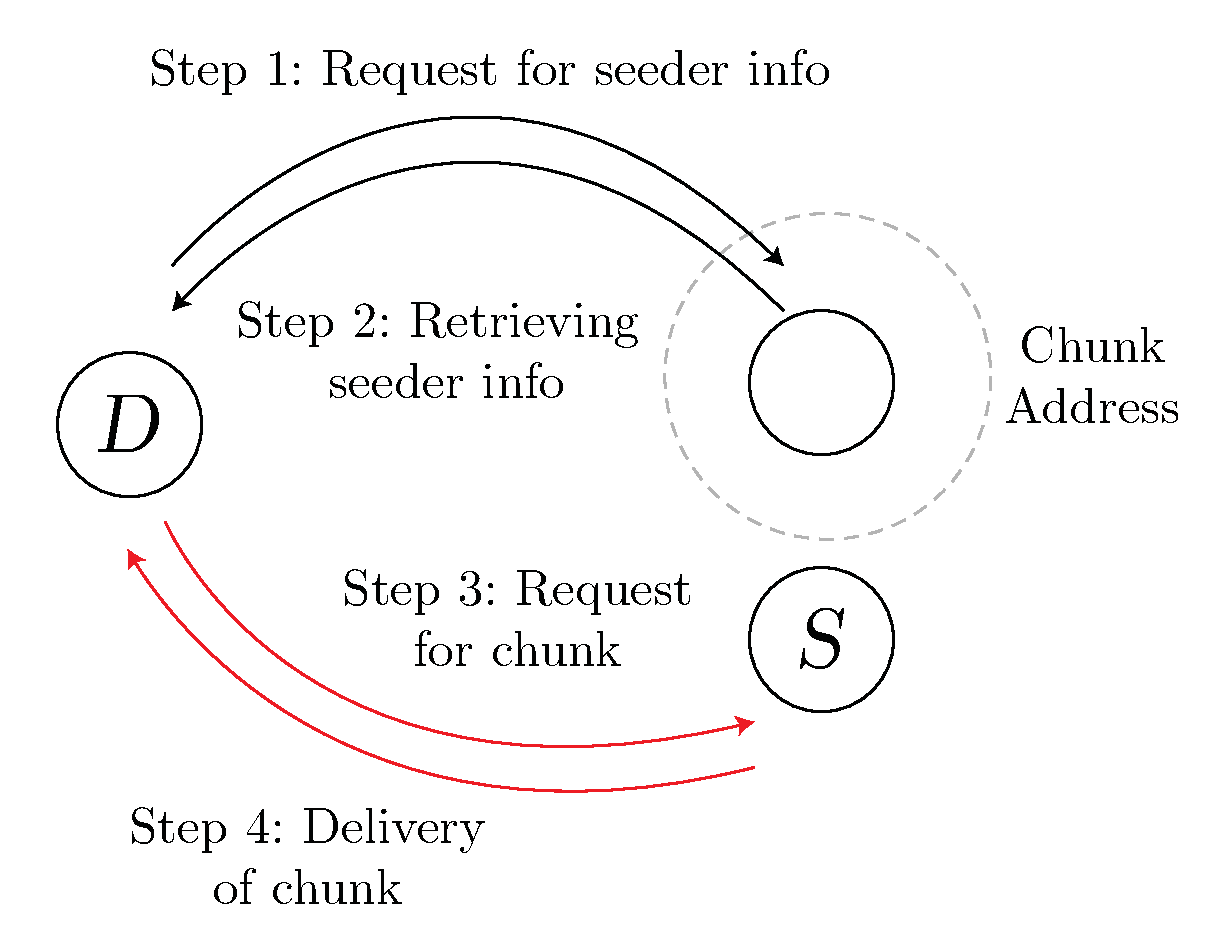
\includegraphics[width=\linewidth]{figs/dht.pdf}
        \caption{}
        \label{fig:dht}
    \end{subfigure}
    \hfill
    \begin{subfigure}{0.5\textwidth}
        \centering
        \raisebox{40pt}{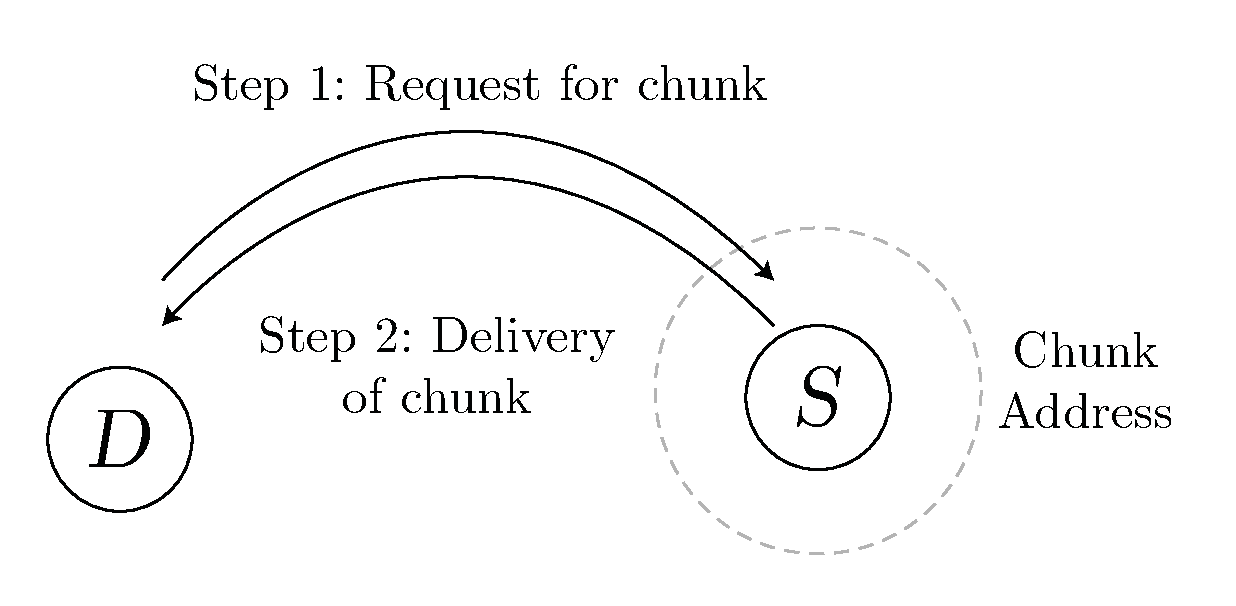
\includegraphics[width=\linewidth]{figs/disc.pdf}} 
        \caption{}
        \label{fig:disc}
    \end{subfigure}
    \caption{Content discovery and retrieval in (a) DHT (b) DISC.}
    \label{fig:content_discovery}
\end{figure}

Fig. \ref{fig:content_discovery} illustrates the process of content discovery and retrieval. The described model can be really effective in large networks since the content is retrieved immediately after locating the closest node, eliminating additional connections and reducing latency. In the simplest case where the closest node is a peer, the retrieval process is reduced to one routing request. On the contrary, a node in IPFS would have to query the DHT twice (see paragraph \ref{par:retrieving_ipfs}) in order to obtain the identity and the addresses of the node that can provide the content and then establish a connection to retrieve it. 

\paragraph{Forwarding \& Backwarding Kademlia}\label{par:forwarding_kademlia}
Most peer-to-peer networks use implementations of the Kademlia protocol that are based on iterative routing for data lookup. Such an implementation is employed by IPFS and is briefly described in paragraph \ref{par:retrieving_ipfs}. However, there are variants of the Kademlia in the literature, for instance R/Kademlia, Pastry and Bamboo \citep{chowdhury_2017},  which use recursive routing to achieve higher performance, reduce latency and bandwith consumption \citep{heep_2010}.

Swarm utilizes a recursive routing protocol which is termed as \textit{forwarding} Kademlia and was outlined by \cite{tron_2018}. In this approach, \hl{instead of receiving references back to closer nodes}, the initial request by a node is forwarded by its peers to nodes closer to the data's identifier. Particularly, each node passes the request to a direct peer, i.e. a peer with who they maintain an active connection, that is at least one step closer to the destination in terms of PO. This process continues until the closest node is found.

The DISC (see paragraph \ref{par:disc}) model suggests that content is to be found with nodes closer to its address. In the described routing approach, when a retrieval request reaches its destination (storage node), the response (requested data) is routed back along the same path; the same intermediate nodes pass the delivery back towards the original requestor. This routing method, \hl{for obvious reasons}, is called \textit{backwarding} Kademlia.

Swarm's Kademlia variant facilitates the following important properties:

\begin{itemize}
    \item \textbf{Automatic availability scaling with increased demand}: Nodes involved in fowarding and backwarding chunks, cache them in an opportunistic manner (see paragraph \ref{par:caching_swarm}), thereby increasing availability and facilitating faster access if the same data is requested again. This automatically scales with popular content. 
    \item \textbf{Privacy and Permissionless Interaction}: In the iterative method, the requestor establishes a connection with each node that takes part in the routing process, disclosing their identity. In forwarding Kademlia, the original request appears identical to any request from an intermediate node, thus promoting privacy by protecting the identity of the requestor.
    \item \textbf{Effectiveness (High performance low latency)}: Forwarding Kademlia, in contrast to the iterative method, decreases network traffic by not relying on the online status of known peers. Nodes always forward requests to connected peers. So, there is no need for back-and-forth communication in order to find new seeders when targeted ones leave the network, as in the iterative approach.
\end{itemize}

Overall, Swarm's implementation of forwarding-backwarding Kademlia improves the network's scalability, reduces bandwidth usage and latency, and strengthens user privacy.

\paragraph{Upload and Redundancy}\label{par:upload_swarm}
When data is uploaded to Swarm it is split into chunks, stored in the uploader's local storage and then disseminated into the network via the \textit{push-sync} protocol \citep{swarm_team_2021}. This protocol is responsible for routing a chunk of data to its destination, that is, a storage node whose address is the closest to the chunk's address.

The chunk is forwarded by intermediate nodes along the same route that a retrieval request would take. Once the chunk reaches its destination, a \textit{statement of custody receipt} is sent back along the same path so that uploaders can ensure that their upload is globally retrievable before sharing the content's address \citep[p.~47]{tron_2020}. Just like the retrieval process, all nodes that forward the chunk to its destination do so via identical messages, which leads to anonymous uploading.

However, if the closest node is the only host of a piece of data and it leaves the network, then there is no way to retrieve the content. To ensure redundancy the \textit{pull-sync} protocol was introduced \citep{swarm_team_2021}. This protocol is highly connected to the notion of \textit{responsibility}.

The radius of responsibility \textit{r} of a node is the smallest PO such that the node is connected to all other nodes in the network that have a PO higher than \textit{r}. Nodes in Swarm are responsible for storing and serving chunks whose addresses fall within their radius of responsibility, i.e a chunk's address shares a number \hl{x >= r} of leading bits with the node's address.

The pull-sync protocol aims to sync chunks within a neighborhood of responsibility, as well as maximize resource utilization in the network by pushing chunks to nodes with excess storage. In short, when two nodes connect, they start sharing chunks in both directions. As a result, nodes in a neighborhood eventually replicate all chunks for which they are responsible. Also note that the pull-sync protocol maintains consistency in the neighborhoods as the topology changes (old nodes leave and new ones join).

Therefore, while the push-sync protocol ensures that chunks are initially stored in the right neighborhood, the pull-sync protocol maintains redundancy and consistency in the neighborhood, even as nodes join or leave the network. \sout{For instance, the push sync protocol pushes chunks to nodes in the neighborhood of the chunk's address, and the pull sync protocol ensures that nodes in a neighborhood pull chunks from each other to keep their storages in sync}. The replication of chunks makes the network more resilient as it enhances their availability.

\paragraph{Caching}\label{par:caching_swarm}
Swarm has adopted an opportunistic caching mechanism where forwarding nodes \hl{(nodes that pass chunks to other nodes)} cache chunks they receive and relay in case they are requested again \citep[p.~47]{tron_2020}. More specifically, nodes in Swarm cache:

\begin{itemize}
    \item \textbf{Downloaded chunks}: Nodes cache chunks that they explicitly download.
    \item \textbf{Uploaded chunks}: Nodes cache chunks that they explicitly upload.
    \item \textbf{Requested chunks}: When a retrieval request is made, the desired chunks are forwarded from node to node until they reach the recipient \hl{(requesting node)}. All intermediate nodes cache the chunks.
    \item \textbf{Push-synced chunks}: During the upload process chunks are forwarded until they reach their neighborhood of responsibility. All intermediate nodes cache the chunk.
\end{itemize} 

Nodes in the Swarm network store and serve chunks of data but unlike IPFS, are rewarded for their contribution. They receive a reward every time they serve a chunk. The profitability of a chunk is proportional to its popularity; the more often a chunk is requested, the higher the reward. Accordingly, the garbage collection method used takes into account the profitability factor, which is reasonably determined by the age of the last request (Least Recently Used (LRU) strategy) \citep[p.~72]{tron_2020}. Thus non-popular chunks are more likely to be removed, creating an auto-scaled content distribution network \citep[p.~72]{tron_2020} where popular chunks become more widely spread and much faster to retrieve. This helps optimize the overall performance and efficiency of the network.

Finally, Swarm has also adopted the concept of pinning which protects content against garbage collection, forcing the node to keep it permanently in its local storage. In contrast to IPFS, local pinning is not enough to ensure that a chunk is generally retrievable by other nodes since the pinner might not be in the neighborhood of responsibility where the chunk is meant to be stored. In order to overcome this, global pinning and a recovery process are proposed where pinners re-upload the missing chunk and then serve it to the requester \citep[pp.~161--167]{tron_2020}.

In summary, the automatic caching we described is aided by Swarm's content routing mechanism, which forwards data through the network both during upload and download, and facilitates low latency data retrieval, availability, and robustness against failures. Apparently, popular data which is requested frequently is favored by the caching mechanism. However, even data missing from their neighborhood of responsibility can be retrieved through the recovery process.

\subsection{IPFS \& Swarm Side-by-Side}\label{sec:ipfs_vs_swarm}
% \subsection{Overview of IPFS and Swarm as decentralized storage solutions (IPFS vs Swarm)}\label{sec:}
In this section, we present a side-by-side comparison of IPFS and Swarm emphasizing mainly their differences. By clarifying their distinct architectural and design choices, we aim to offer \hl{comprehensive/broader} overview and a better understanding of how each system achieves data availability, content addressing, censorship resistance, etc.

Content is split into chunks before being uploaded to either of these platforms. A chunk is a piece of data that represents the basic unit of storage and retrieval in IPFS and Swarm. Each chunk is uniquely referenced using its cryptographic hash to achieve content addressing instead of the widely used location addressing. This allows for quick verification of received data and enables deduplication. In Swarm, a Binary Merkle Tree (BMT)  \citep{tron_2020} hash algorithm based on Keccak-256 is used to generate the identifiers of the chunks. Note that for encrypted content, the identifier is the concatenation of the chunk hash and the decryption key and therefore is represented in 64 bytes. The developers of IPFS approached this matter differently to provide more flexibility to end users. They introduced CID  \citep{multiformat}, a self-describing upgradable content-addressed identifier, which consists of the hash digest of the content and some metadata as a prefix. From the metadata, the CID version and its encoding, as well as the hashing function used and the content’s type can be determined.

In order to \emph{``group''} chunks of the same data together, both platforms implement some sort of tree data structure. The root hash of such trees refers to the data as a whole. In IPFS a Merkle Directed Acyclic Graph (DAG)  \citep{benet_2014}, a generalized construction of a Merkle Tree, is used. It allows nodes to have multiple parents, does not need to be balanced, and non-leaf nodes can contain data. Swarm once more embraced the use of Merkle Trees, in which intermediate nodes contain links to leaf nodes that hold the chunks. In the case of uploading folders, IPFS recursively constructs a Merkle DAG, whereas Swarm utilizes a Trie  \citep{tron_2020} data structure. Both these schemes allow for Unix-like path resolving.

Another fundamental difference between IPFS and Swarm lies in what content participating nodes in each network store. In the former, a node holds content depending on its interests, while in the latter a \emph{``cloud''} is formed with every node storing arbitrary chunks of data originating from other nodes \citep{swarmwiki_2019}. In both cases, nodes also cache content they access, until it is \emph{``garbage collected''}. This mechanism is crucial in ensuring that the distribution of popular content scales automatically and retrieval latency is decreased. Swarm takes this one step further by implementing an opportunistic cache model: intermediate nodes cache all chunks they forward.

Moreover, the subjects at hand approach data discoverability and retrieval differently. In IPFS a distributed hash table (DHT) \citep{benet_2014} is used to map CIDs to seeders that can serve that content. In Swarm, a similar model called DISC  \citep{tron_2020} was developed, in which content (value) is directly stored under a corresponding identifier (key), potentially reducing the retrieval process to one routing request. Besides that, in both platforms data are public by default. However, Swarm offers the choice of encrypting data before an upload. Finally, Swarm has a built-in incentive system based on Ethereum, while IPFS depends on a separate blockchain, Filecoin. 

\section{Related work - Purpose and significance of the thesis}\label{sec:related_work}
There are tools for assisting developers to minimize gas consumption, but mostly, the focus is on the program structures rather than the data  \citep{nelaturu_2021, chen_2017, chen_2021}. Among them, we singled out Gasper  \citep{chen_2017}, a cost minimization tool that analyzes bytecode to determine costly patterns in SCs. Its creators used it to analyze approximately 4000 SCs and concluded that three of these patterns were found in the majority of them. This research was continued, and new patterns have been added  \citep{chen_2021}. There is also work on parametric cost bounds in the Ethereum blockchain \citep{albert_2021}.

Data storage cost and gas-saving methods are studied to some extent in the context of specific use cases  \citep{kurt_2020, delgado_2019, westerkamp_2020}. Gas consumption of SCs is examined in  \citep{grech_2020, signer_2018}, but none of them researches the related cost holistically by considering all possible ways of using Ethereum as a data store. In  \citep{consensys}, the use of events as an alternative data storage option was proposed. However, the novel idea of storing data in a transaction’s payload is barely studied. Blockchi \citep{yankov_2018} is a tool that allows storing and retrieving JSON objects, while in  \citep{xie_2017} a storage model is proposed for storing data from IoT sensors in hexadecimal format. In the latter, transaction references are retained in an external database. In our work, apart from evaluating the transaction payload as a data store, we propose an extension to this approach, which we term as \emph{``Unused Function Parameters''}. In short, it is a means of storing data in a transaction's payload while exploiting Solidity's built-in ABI interface to allow handling all available data types.

A common architecture for managing large chunks of data is to use distributed file systems such as IPFS and Swarm for storage and record the resulting content identifiers in Ethereum. This approach has been studied in several applications, e.g., \citep{hao_j_2018, ren_2021}, but no comments were made on the performance of these platforms nor on the cost of recording the content identifiers. Ramesh et al.\cite{ramesh_2019}, exploited such a scheme to handle IoT data and also studied both local retrieval and upload performances of IPFS and Swarm. In \citep{shen_2019}, IPFS was evaluated for remote and local retrieval latency. In \citep{abdullah_2021} the performance of IPFS in a private network was compared to that of FTP. Furthermore, a recent study conducted by Ismail et al. \cite{aisyah_2022} reviewed several works centered around the performance of distributed file systems. In light of the available literature, it is apparent that the majority of attention is being directed towards IPFS, leading us to believe that Swarm’s performance is an under-researched topic. On top of that, it's worth mentioning that research on Swarm's performance prior to three years ago should now be considered outdated, as a new client \citep{swarm_bee} and updates to the underlying protocols were introduced in 2020 \citep{tron_2020}. Our work is focused on local read-write performance of IPFS and Swarm, and the cost associated with storing the corresponding content identifiers in Ethereum.

In conclusion, even though the necessity of minimizing gas consumption is recognized in the literature, existing studies focus mainly on program structures or inefficient patterns. At the same time, efficient data management is an under-researched topic despite the fact that it is an essential part of DApps. In this work, through the research question we posed and the corresponding research we conducted, we intend to give a comprehensive perspective on efficient ways of handling data both on-chain and in hybrid architectures.

\subsection{Existing data management approaches in Ethereum-based dApps}\label{subsection:}
\subsection{Cost and retrieval performance of the aforesaid approaches}\label{subsection:}
\subsection{Cost and retrieval performance of the hybrid approaches}\label{subsection:}
\subsection{Purpose and significance of the thesis}\label{subsection:}

